\فصل{الگوریتم‌های پیاده سازی شده}

\section{نگاشتی بر اساس سیستم بینایی انسان}
سیستم بینایی انسان، برای دیدن جزئیات در نورهای مختلف، و ساخت یک تصویر درست در ذهن
\lr{ذهن}\footnote{\lr{percept}}
، به روش های مختلفی خود را سازگار می کند.
 در این روش سعی می کنیم برای نزدیک کردن تصویر خروجی به تصویر واقعی یا تصویری که چشم ما از منظره درک می کند، سازگاری های انجام شده توسط سیستم بینایی انسان را توسط کامپیوتر شبیه سازی کنیم. 
 
 اولین مرحله‌ی سازگاری در سیستم بینایی، در مردمک چشم صورت می‌گیرد که اندازه ی خود را با توجه به میزان روشنایی کلی که وارد چشم می‌شود تنظیم می کند. در مرحله‌ی دوم، شبکیه‌ی چشم میزان حساسیتشان را به میانگین روشنایی وارده تغییر می دهند. در مرحله ی سوم، یک سازگاری محلی برای مشخص کردن تضاد به وجود آمده در قسمت‌های متفاوت تصویر با توجه به محل خیره شدن انجام می شود.
 
در این بخش روشی برای ارائه‌ی تصاویر با دامنه‌ی دینامیکی بالا ارائه می شود، که برگرفته از نگاشت‌های سراسری و محلی‌ای است که در سیستم بینایی انسان انجام می شود. 

از مزایای این روش، استفاده از نگاشت محلی با توجه به شکل لبه‌های با تضاد روشنایی بالا است. این موضوع خود باعث کاهش هاله های مصنوعی که در اثر نگاشت‌های محلی به وجود می‌آید می‌شود.
همچنین در این روش،  روشنایی تصویر  چداگانه پردازش می شود. برای این کار روشنایی را با استفاده از آنالیز مولفه‌های اصلی محاسبه می کنیم که تعامد روشنایی و کانال‌های رنگ را به حداکثر برسانیم. در نتیجه، در اثر این نگاشت، تغییر رنگ کمتری در تصویر ایجاد می شود.

کلیات این نگاشت به این صورت است که ابتدا تصویر روشنایی را تفکیک می کنیم. روی تصویر روشنایی، یک مرحله نگاشت سراسری، و پس از آن یک نگاشت محلی اجرا می کنیم. به صورت موازی، روی تصویر رنگی نیز یک نگاشت سراسری اجرا می کنیم. و در نهایت این دو تصویر را با هم ترکیب می کنیم.
\begin{figure}[!htb]
	\minipage{1\textwidth}
	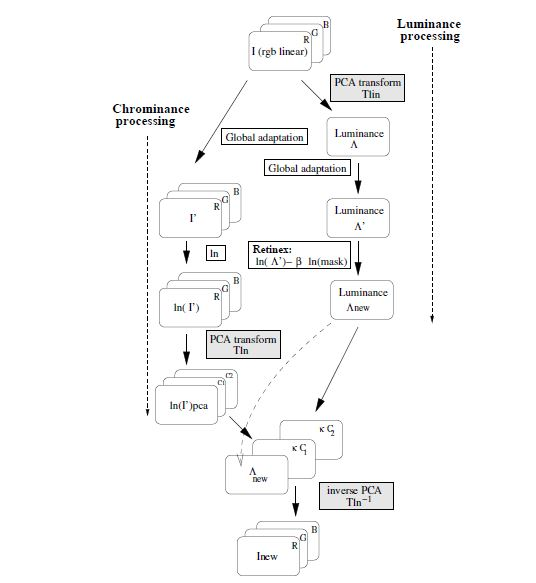
\includegraphics[width=\linewidth]{images/retinexbigpic}
	\caption{}\label{fig:logtonemap}
	\endminipage\hfill
	%	
	%	\centerline{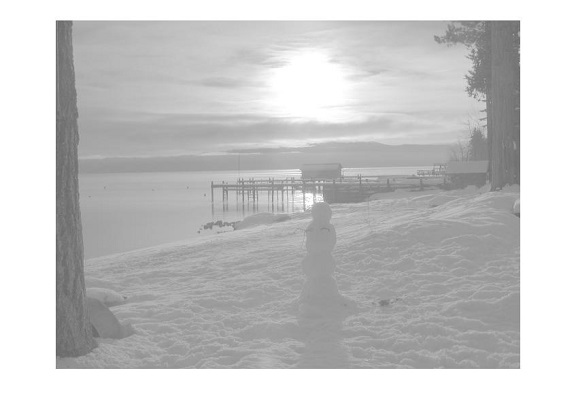
\includegraphics{images/retinexglobal}}
\end{figure}

در این بخش به مراحل پیاده سازی و اچرای این الگوریتم می پردازیم.

\subsection{نگاشت سراسری}
در این قسمت، فشرده‌سازی اولیه ی دامنه، روی تصویر اجرا می‌شود، این فشرده‌سازی، در واقع کاری که مردمک چشم انجام می‌دهد را شبیه سازی می‌کند.این شبیه‌سازی، می‌تواند توسط یک تابع نمایی انجام شود.انحنا‌ی تابع نمایی‌ای که این نگاشت را تقریب می‌زند، به میانگین روشنایی عکس وابسته است.

برای محاسبه‌ی روشنایی، از اولین مولفه‌ی اصلی که روی محور 
\متن‌لاتین{RGB }
 به دست می‌آید استفاده می کنیم. به این ترتیب، روشنایی بیشترین استقلال ممکن را نسبت به رنگ‌ها دارد، و پردازش روشنایی مستقل از رنگ‌ها به خوبی انجام می‌شود.
 
 \begin{code}
 \begin{matlab}
 	 flatimage = reshape(image, [N 3]);
 	 coeff = princomp(flatHDR);
 	 PsiCoeff = [coeff(:, Gcoeff)];
 	 Psi = zeros(n, m);
 	 %R,G and B are first, second, and thired column of HDR image
 	 %representing red, green and blue channels respectively
 	 Psi(:,:) = R * PsiCoeff(1, 1) + G * PsiCoeff(2, 1) + B * PsiCoeff(3, 1);
 \end{matlab}
 %\caption{نمونه کد متلب}
 \end{code}


اکنون $\Lambda$ روشنایی محاسبه شده برای عکس توسط مولفه‌ی اصلی تصویر
\متن‌لاتین{RGB }
است. میانگین روشنایی از طریق رابطه‌ی زیر قابل محاسبه است که در آن $N$ تعداد پیکسل‌های موجود در تصویراست.

\begin{equation}
	\Lambda_{av} = \frac{\varSigma ln(\Lambda(p))}{N}
\end{equation}

روشنایی نهایی، از طریق رابطه‌ی زیر قابل محاسبه است.

\begin{equation}
	\Lambda^{'}(p) = \Lambda^{\frac{1}{\gamma}}	
\end{equation}

$\frac{1}{\gamma}$
در رابطه ی بالا،  یک تابع مستوی از  روشنایی میانگین است که از طریق زیر به دست می آید. این ضرایب به صورت تجربی به دست آمده اند.

\begin{equation}
	\frac{1}{\gamma} = min(1, \frac{1}{6} \Lambda_{av} + \frac{1}{3})
\end{equation}

تصویر زیر، توسط این نگاشت به وجود آمده است. همان طور که می بینید، در تصویر بخش های سفید و سیاه، به خوبی نشان داده نشده اند. البته رنگی نبودن آن، به خاطر این است که در این نگاشت فقط روشنایی عکس را مورد پردازش قرار داده ایم.

 
 \begin{figure}[!htb]
 		\minipage{1\textwidth}
 		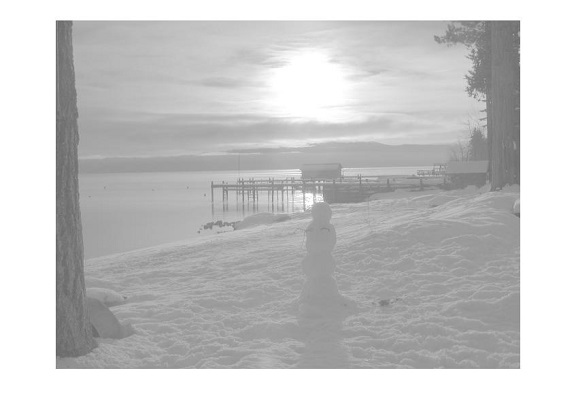
\includegraphics[width=\linewidth]{images/retinexglobal}
 		\caption{}\label{fig:logtonemap}
 		\endminipage\hfill
 		%	
 %	\centerline{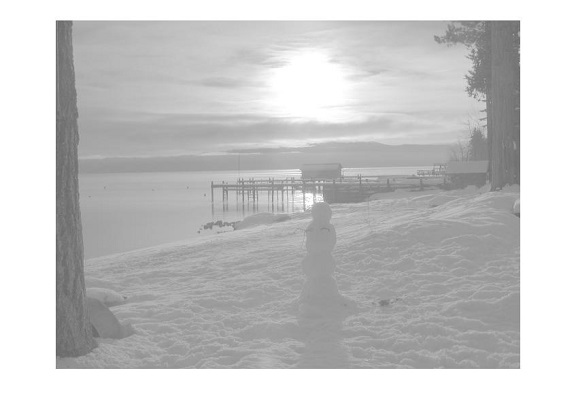
\includegraphics{images/retinexglobal}}
 \end{figure}
 
 
\subsection{نگاشت محلی}

پس از نگاشت سراسری که روی تصویر انجام می‌شود، یک نگاشت محلی برای افزایش وضوح جزئیات صورت می‌گیرد.

نگاشت محلی که در این الگوریتم در نظر گرفته شده، یک نگاشت 
\متن‌لاتین{surround-based }
  است، به  این معنی که به هر پیکسل، یک مقدار جدید، با توجه به پیکسل‌های احاطه‌گر آن اختصاص می دهد.معمولا در این الگوریتم‌ها از اختلاف بین مقدار هر پیکسل، و یک ماسک که میانگین وزن‌دار پیکسل‌های احاطه گر آن است، استفاده می‌شود.
  


\begin{equation}
	\Lambda^{"} = ln(\Lambda^{'}(p)) - ln(mask(p))
\end{equation}

\subsubsection{اصلاح بخش سیاه و سفید}
امامشکل این رابطه، این است که بخش‌های سیاه تصویر، کاملا سیاه نمی‌مانند، و بخش‌های سفید نیزکمی تیره می‌شوند.برای رفع این مشکل، یک متغیر $ \beta$ تعریف می‌کنیم، که این تبدیل‌ رابهبود ببخشد.


\begin{equation}
	\Lambda^{"} = ln(\Lambda^{'}(p)) - \beta ln(mask(p))
\end{equation}

رای محاسبه‌ی این رابطه، با توجه به این که $mask$ و $\Lambda$ هر دو در بازه‌‌ی [0,1] هستند، آن‌ها را به مقیاس [0.1,100] نگاشت می‌دهیم , مقادیر جدید آن ها را به ترتیب $mask_{ln}$ و $\Lambda^{'}_{ln}$ می نامیم. این مقادیر از طریق روابط زیر قابل محاسبه اند. البته لگاریتم طبیعی در بازه ی مشخص شده، از طریق تابع نمایی $\frac{1}{3}$ نیز قابل تقریب زدن است.


\begin{equation}
	\Lambda^{'}_{ln} = \frac{1}{ln(100)}.ln(max(0.1, \Lambda^{'}(p)\times 100))
\end{equation}	

\begin{equation}	
	mask^{'}_{ln} = \frac{1}{ln(100)}.ln(max(0.1, mask^{'}(p)\times 100))	
\end{equation}

به این ترتیب، رابطه‌ی فوق به شکل زیر بازنویسی می‌شود.


\begin{equation}
	\Lambda^{"} = \Lambda^{'}_{ln}(p) - \beta mask_{ln}(p)
\end{equation}
حال به ضریب بتا می‌پردازیم.
این ضریب به  صورت یک تابع سیگموئید و به گونه‌ای تعریف شده‌است که برای مقادیر با روشنایی شدید، ضریب نزدیک به صفر باشد، تا با کم شدن مقدار 
\متن‌لاتین{$ \beta mask_{ln}(p) $ }
از مقدار خود پیکسل، روشنایی کمتر نشود. همچنین برای مقادیر با روشنایی کم، این ضریب نزدیک به یک می‌باشد که به این ترتیب، این مقدار، همچنان تیره می‌ماند. این ضریب، از طریق رابطه زیر قابل محاسبه است.


\begin{equation}
	\beta = 1 - \frac{1}{1 + e^{-10.(max(0, \Lambda^{'}_{ln}(p)) - 0.5))}}
\end{equation}

حال باید اعداد را به مقیاس اصلی باز گردانیم، ضمنا با توجه به این که ممکن است در این میان عددی منفی شود، طبق بحث صورت گرفته در بخش 2.2، رابطه‌ی بالا را به صورت زیر اصلاح می‌کنیم.

\begin{equation}
	\Lambda_{new} = min(1, \frac{max(0, \Lambda^{"}(p) - b)}{\omega - b}) 
\end{equation}

\subsubsection{معضل هاله‌های مصنوعی  }

یکی دیگر از معضلات این روش، معضل انتخاب بین ارائه‌ی خوب تصویر، و افزایش وضوح جزئیات در تصویر است. اگر پیکسل‌های احاطه‌گر را کوچک در نظر بگیریم، به صورت محلی وضوح تصویر بالا می‌رود، اما باعث ایجاد هاله‌های مصنوعی می‌شود.استفاده از فضای احاطه‌گر بیشتر، هاله‌های مصنوعی را کاهش می‌دهد، اما تضادها را کاهش داده، و در نتیجه وضوح تصویر را کاهش می‌دهد.
در این الگوریتم، برای مقابله با مشکل هاله‌های مصنوعی، فضای احاطه‌گر را ثابت در نظر نگرفته، و آن راسازگار با لبه‌های با تضاد روشنایی شدید تعریف می‌کنیم. به این ترتیب، بخش‌های روشن نامربوط، روی روشنایی بخش‌های تاریک تصویر تاثیرگذار نمی‌شوند و بالعکس. 
برای مشخص کردن گوشه‌ها، از الگوریتم $canny$ استفاده می‌کنیم.

با توجه به مطرح شدن گوشه‌ها،  محاسبه‌ی $mask$ برای هر کدام از پیکسل‌ها باید به صورت جداگانه صورت گیرد. به طور کلی $mask$ میانگین وزن‌دار میزان روشنایی فضای احاطه‌گر تعریف شده برای هر پیکسل است. این مقدار از طریق رابطه‌ی زیر قابل محاسبه است. 

\begin{equation}
	mask(x,y) = \frac
	{\sum_{\theta=0}^{360}\sum_{r=0}^{r_{max}}
		\Lambda'\big(x+r.\cos(\theta), y+r.\sin(\theta) \big).e^{-\frac{r^2}{\sigma_{\theta,r}^2}}}
	{\sum_{\theta=0}^{360}\sum_{r=0}^{r_{max}}e^{-\frac{r^2}{\sigma_{\theta,r}^2}}}
\end{equation}

 
 که در آن 
 \متن‌لاتین{(x,y) }
 نشان‌دهنده‌ی مختصات پیکسل
  \متن‌لاتین{p } ، 
  \متن‌لاتین{$ \theta $ }
 زاویه‌ای که یک پیکسل در فضای احاطه‌گر با 
  \متن‌لاتین{p } 
 می‌سازد، و 
  \متن‌لاتین{r }
 فاصله  با
  \متن‌لاتین{p } 
   است.
 
 همچنین مقدار  
   \متن‌لاتین{$\sigma$}
  در صورتی که  یک گوشه با تضاد روشنایی بالا از آن عبور نکرده باشد، برابر با 
   \متن‌لاتین{$\sigma_{0}$}
   و در غیر این صورت برابر با 
   \متن‌لاتین{$\sigma_{1}$}
   است.
این مقادیر به صورت تجربی برابر $\frac{1}{16} $و $\frac{1}{8} $در نظر گرفته می شوند.
 %todo
 
 \subsubsection{یافتن لبه‌ها }
 
 همان‌طور که پیش تر گفته شد، برای یافتن لبه‌ها با تضاد روشنایی بالا، از الگوریتم 
  \متن‌لاتین{canny }
 استفاده می‌کنیم.
 این الگوریتم لبه‌ها را با توجه به بیشینه‌های محلی شیب تصویر، پیدا می‌کند. لبه‌های ضعیف و قوی را مشخص می‌کند. اگر لبه‌ای ضعیف باشد، تنها در صورتی آن را نمایش می‌دهد که به یک لبه‌ی قوی متصل باشد. آستانه‌ای که تفاوت لبه‌ی ضعیف و قوی را مشخص کند، در تمام تصویر‌ها یک مقدار ثابت است که به صورت تجربی به دست آمده است. به این ترتیب، ممکن است برای تصویر‌هایی که لبه‌ای با تضادروشنایی نسبتا بالا ندارند، هیچ لبه‌ای تشخیص داده نشود.
 در پایین، چند نمونه از تصاویر سیاه و سفید و لبه های تشخیص داده شده برای آن ها با الگوریتم 
   \متن‌لاتین{canny }
 را مشاهده می کنید. همان طور که گفته شد، الگوریتم مورد بحث، روشنایی را از رنگ جدا می کند، در نتیجه به طور خودکار در این مرحله، تصویری که داریم سیاه و سفید است.
  \begin{figure}[!htb]
  		\minipage{1\textwidth}
  		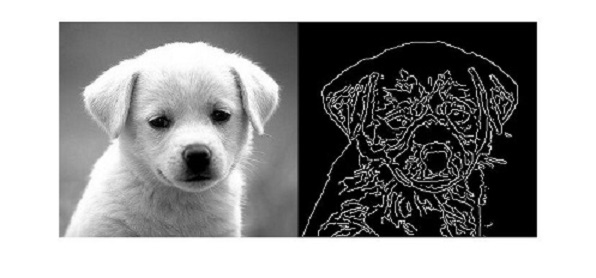
\includegraphics[width=\linewidth]{images/cannyexample1}
  		\caption{}\label{fig:logtonemap}
  		\endminipage\hfill
  %	\centerline{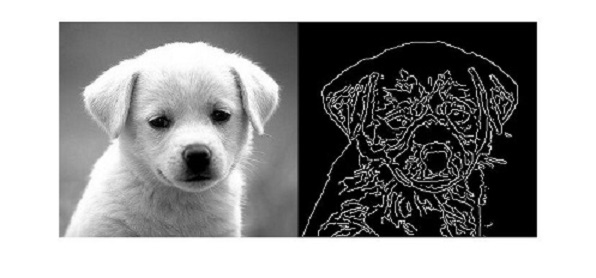
\includegraphics{images/cannyexample1}}
  \end{figure}
  
   
   \begin{figure}[!htb]
   		\minipage{1\textwidth}
   		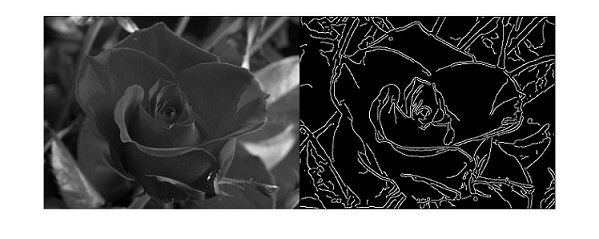
\includegraphics[width=\linewidth]{images/cannyexample2}
   		\caption{}\label{fig:logtonemap}
   		\endminipage\hfill
  % 	\centerline{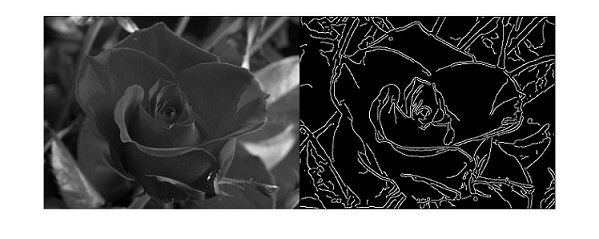
\includegraphics{images/cannyexample2}}
   \end{figure}
   
 
\subsection{پردازش رنگ}
برای پردازش رنگ تصویر، دقیقا مراحلی که در پردازش تصویر روشنایی انجام دادیم را روی هر کدام از کانال‌های رنگی تکرار می‌کنیم، با این تفاوت که نگاشت محلی را انجام نمی‌دهیم.

نگاشت سراسری ای که در بخش قبل گفته شد روی هر کدام از 
 \متن‌لاتین{R }،
  \متن‌لاتین{G } و 
   \متن‌لاتین{B }
 تصویر 
    \متن‌لاتین{I }
  اجرا می‌شود تا تصویر 
     \متن‌لاتین{$I^{'}$ }
  ایجاد شود.
  از مقادیر لگاریتم می‌گیریم . اولین مولفه‌ی اصلی این مقادیر را محاسبه می کنیم تا 
$\ln(I')_{pca}$              
    به دست بیاید. این مقدار را با
$\Lambda_{new}$
   جایگذاری می کنیم. همان طور که قبل تر هم اشاره شد، مولفه ی اول $PCA$ نمایش گر نور، و مولفه های دوم و سوم، به ترتیب نمایشگر زرد -آبی  و قرمز-سبز هستند.
   
   حال تصویر را باز سازی می کنیم. 
   برای این کار  ماتریس تصویر را در فضای $PCA$به شکل زیر می‌سازیم.
   
   ستون اول ماتریس، روشنایی تصویر است که در بخش قبل محاسبه شد. ستون دوم و سوم به ترتیب مولفه‌های دوم و سوم $PCA$ هستند. حال کافی است از یک تبدیل برای انتقال تصویر از فضای $PCA$ به فضای $RGB$ استفاده کرد تا تصویر نهایی در قالب $RGB$ ایجاد شود.
   
    
    \begin{code}
    	\begin{matlab}
    		 % change matrix represenation into vector representation
    		 b1 = PCA(:,:,1);
    		 b2 = PCA(:,:,2);
    		 b3 = PCA(:,:,3);
    		 b_vec = cat(2,b1(:),b2(:),b3(:));	 
    		 % apply transformation
    		 RGB_vec = b_vec*inv(V);
    	\end{matlab}
    	%\caption{نمونه کد متلب}
    \end{code}
    
  
  

\section{نگاشت 
	\متن‌لاتین{reinhard }
}

در این روش، ابتدا یک نگاشت اولیه‌ی سراسری اعمال می‌کنیم. این نگاشت با استفاده از سیستم zone که در ادامه تعریف می‌شود انجام می‌شود. پس از این نگاشت، در صورت نیاز، یک اصلاح محلی به نام  dodging and burning انجام می‌شود.
%todo


\subsection{نگاشت سراسری}
کلید یک تصویر، نشان‌دهنده‌ی ذهنیت ما نسبت به میزان روشنایی کلی یک تصویر است. به عنوان مثال برای یک دیوار سفید، دارای مقدار کلید بالا، و مقدار کلید یک دیوار سیاه، کوچک است.
یک روش ساده برای توصیف این مقدار استفاده از کدگذاری
\متن‌لاتین{log-average luminance }
است، که از طریق رابطه‌ی زیر قابل مقایسه است.

\begin{equation}
	\overline L_{w} = \frac{1}{N} \exp (\sum_{x,y} \log(\sigma + L_{w}(x,y))) 
\end{equation}

در این رابطه، 
\متن‌لاتین{L(x,y)}
میزان روشنایی تصویر در پیکسل 
\متن‌لاتین{(x,y) }
است، و $\sigma$ یک مقدار کوچک است که برای جلوگیری از یکپارچه شدن تصویر اضافه می‌شود. این یکپارچگی رنگ، در صورت وجود نقاط سیاه در تصویر به وجود می‌آید.
خواسته‌ی ما این است که پیکسل با روشنایی میانگین( که در بالا محاسبه شده است) را به $middle-gray$ یا مقدار 0.18 نگاشت دهیم. به این ترتیب رابطه‌ی زیر را داریم. 

\begin{equation}
	L(x,y) = \frac{a}{\overline{L_{w}}}L_{w}(x,y)
\end{equation}

با تغییر مقدار   $a$ می‌توان میزان روشنایی را تغییر داد، این میزان را کاربر می‌تواند خود انتخاب کند، زیرا همان طور که مشخص است، نگاشت صحیح، معنی ندارد و به هر میزان که کاربر احساس بهتری داشته باشد، نگاشت بهتر است. ما برای پیاده سازی همان طور که گفته شد، مقدار آن را برابر 0.18 قرار دادیم.

تصاویر 3.1 این نگاشت را با استفاده از مقادیر مختلف $a$ نشان می دهد.

\begin{figure}[!htb]
	\minipage{1\textwidth}
	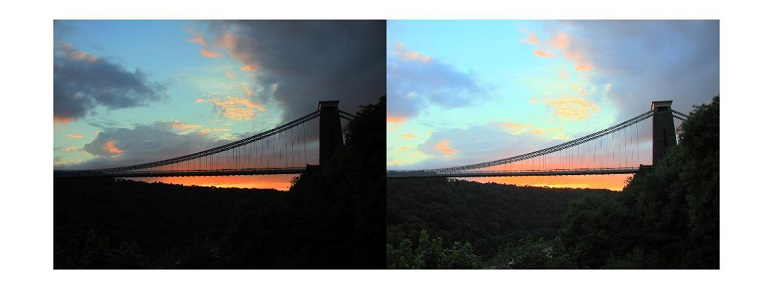
\includegraphics[width=\linewidth]{images/reinharda}
	\caption{}\label{fig:logtonemap}
	\endminipage\hfill
	%	\centerline{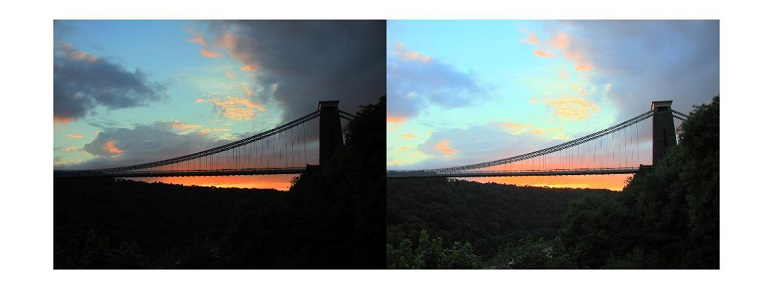
\includegraphics{images/reinharda}}
\end{figure}


نکته‌ای که وجود دارد این است که این گونه خطی نگاشت دادن روشنایی‌ها، عملکرد خوبی ندارد، زیرا تصاویر معمولا دارای رنج روشنایی متوسط هستند که در نقاط خی کمی، روشنایی‌شان از بازه‌ی عادی می‌گذرد. برای حل این مشکل، رابطه‌ی زیر را پیشنهاد می‌کنیم.

\begin{equation}
	L_{d}(x,y) = \frac{L(x,y) (\frac{1+L(x,y)}{L^{2}_{white})}}{1 + L(x,y) }
\end{equation}

که در این رابطه $ L_{white}$کوچک‌ترین مقداری است که می‌خواهیم مقادیر بزرگ تر از آن به سفید نگاشت شوند.

اگر مقدار  $ L_{white}$ را برابر با بی نهایت قرار دهیم، 
\متن‌لاتین{burning } 
اتفاق میفتد. اما اگر مقدار آن را برابر با بیشترین مقدار روشنایی موجود در تصویر قرار دهیم، این مشکل نیز حل می‌شود.

تصاویر 3.2، این نگاشت را با استفاده از مقادیر مختلق برای 
$ L_{white}$ 
نشان می دهد.

\begin{figure}[!htb]
	\minipage{1\textwidth}
	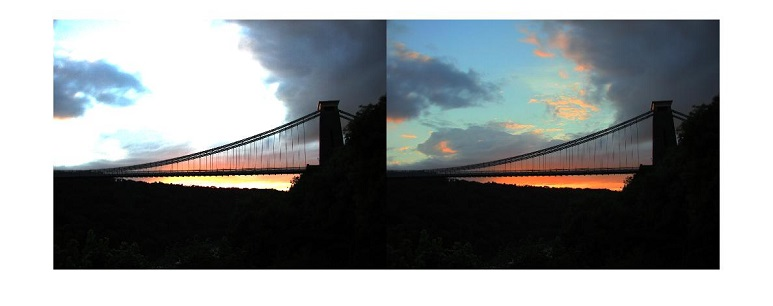
\includegraphics[width=\linewidth]{images/reinhardw}
	\caption{}\label{fig:logtonemap}
	\endminipage\hfill
	%	\centerline{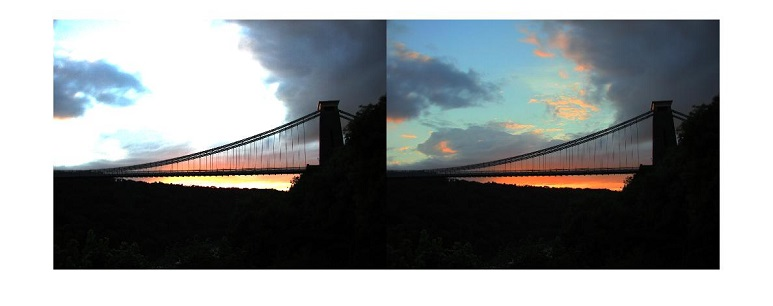
\includegraphics{images/reinhardw}}
\end{figure}


  
 \subsection{نگاشت محلی}
  
